\documentclass{article}
\usepackage[margin=1in]{geometry}
\usepackage{indentfirst}
\usepackage{amsmath,amssymb,amsfonts}
\usepackage{url}
\usepackage{hyperref}
\usepackage{fancyvrb}
\usepackage{graphicx}

\begin{document}

\title{Title}

\author{Alec Olson (ols00160@umn.edu}

% \author{
% \IEEEauthorblockA{}
%     \IEEEauthorblockN{Alec Olson (ols00160@umn.edu)} \\
% }

\maketitle

\section{Domain Problem Statement}
Biomonitoring is an essential tool for invasive species tracking and management, land management, and natural resource conservation and restoration. It is essential for Hennepin County and its partner organizations to know the spatial extent of these species, the severity or density of the infestations, and the stage of treatment or restoration for each area in order to efficiently use the limited time and resources of human field workers to manage these areas.

A particular challenge in invasive species mapping arises due to the inherent limitation of human workers to survey the entire spatial extent of the target area, which can lead to underestimates of the species’ true population and range \cite{https://doi.org/10.1890/0012-9658}. This scarcity of information regarding extent and severity, often combined with multi-year management strategies that can leave areas in varying states of infestation, removal, or restoration, restricts the ability of field workers and policymakers to have full knowledge of the environment \cite{when-to-monitor-or-control}. Further complicating the monitoring and management problem is that many organizations share management responsibilities for a single site, and each organization generally has its own practices and procedures for data collection, making county-wide collaboration challenging.

The field of ecology has methods to deal with the unavoidable limitations of incomplete data collected by field workers \cite{https://doi.org/10.1890/0012-9658} and varying expertise leading to varying quality of data collection \cite{5694101}. However, such methods are statistically and methodologically sophisticated, and not often used in practice. Previous studies have focused on 1) comparing results between UAV- and human-sensed invasive species mapping rather than working in tandem \cite{new-tools-old-problems} \cite{PMID:40775501}; 2) ground-based robots working in structured environments like an agricultural field, not in unstructured environments like a forest \cite{7989612}; and 3) open environments with the vegetation in question visible from the air \cite{new-tools-old-problems} \cite{PMID:40775501}, an approach which will not work in Hennepin County, with its urban environment of buildings, and overpasses that can obstruct drone or satellite imagery and where species such as buckthorn frequently inhabit the understory of forests \cite{mda_common_buckthorn}. Even a 2022 study aiming to use high-resolution satellite imagery to map buckthorn in an urban environment identified limitations to this approach due to the variable distribution densities and proclivity for understory growth of buckthorn \cite{Nininahazwe02102023}.

Furthermore, decision-making regarding prevention, monitoring, treatment, and restoration is complicated by varying phenological properties and behaviors from species to species \cite{review-operations-research-models}. For example, some invasive plants have very similar appearances to their native counterparts, and some invasive plants are most effectively treated at certain times of the year in order to efficiently remove them. However, advancements in the fields of artificial intelligence and robotics offer the possibility to address some of these challenges. In particular, multi-modal AI models that incorporate on-ground robotic sensors, unmanned aerial vehicles (UAVs), and other real-time localized data streams could augment existing skilled human field workers to facilitate more confident decision making regarding invasive species management.


\section{Technical Problem Statement}
Physical AI is one approach that could address these challenges in biomonitoring. Physical AI refers to artificial intelligence systems that, through sensing and interaction with their environment, learn about the physical world around them and can make intelligent decisions accordingly \cite{10.1115/1.4070122}. Such systems can be fully embedded in a single robotics platform or exist across distributed sensing, networking, cloud computing, and actuation platforms, and have applications across industries \cite{10.1115/1.4070122}. Supplementing these systems with natural-language interaction has demonstrated effectiveness in the domain of human-robot interaction by allowing robots to improve their understanding of the world \cite{ahn2022icanisay} \cite{brohan2023rt2visionlanguageactionmodelstransfer} as well as allowing humans to provide natural-language instructions to direct the physical actions of robots \cite{ahn2022icanisay}.


UAVs have been widely researched for use in land management, such as for individual plant segmentation in row crops \cite{10161078} or generating land-cover maps to identify various vegetation types \cite{Ahmed19052017}. However, these assume free range of motion of the UAV because it is required to fly unobstructed over the area of study; this ease of access is not generally possible under the tree canopy or in urban areas due to safety considerations. Buildings, power lines, and communications towers are examples of critical infrastructure that must not be affected by UAVs. 

In addition, ground-based robots face their own challenges while navigating difficult terrain. Thick understory growth, uneven and varying types of ground surfaces, water crossings, and steep slopes are among the difficulties that must be overcome for these robots to be useful in the field. Not only do these represent challenges when designing hardware, but the software must be robust enough to sense what is ahead and determine if it is navigable or not \cite{10876033}.

Previous work has explored how to model spatial crowdsourcing tasks in order to work within a temporal and monetary budget, but these were limited to discrete tasks \cite{10.1007/s00778-019-00568-7}, whereas biomonitoring works in a continuous spatiotemporal environment. The reliability of humans has been modeled before, but in a structured, discrete environment, such as that of image classification with the goal of more accurately determining each image’s label \cite{whose-vote-should-count-more}. Informative path planning, which allows a system to adjust its course of travel based on newly-obtained information in order to visit areas of higher interest, is well-researched but generally assumes a known and constant sensor noise model, such as a Gaussian \cite{informative-path-planning-framework}. Other research into multi-sensor networks to obtain information about the world allows for non-Gaussian noise models but explicitly acknowledges that this is known in advance \cite{mobile-sensor-network-control}, but this assumption cannot be applied to humans \cite{6846739} because their reliability and error rates may exhibit spatiotemporal variability due to terrain, weather, density of vegetation, fatigue, or other factors.

Although these problems have been addressed individually, the integration of them represents a gap in the current literature. A system with an unknown error model that varies in time and space, does not have ground truth data to validate its observations, has both human and robotic components, and which is working in an unstructured, outdoor, ground-based environment is a novel challenge well-suited to physical AI approaches and capabilities.


\section{General Opportunity}
Previous research has attempted to formally model this so-called soft data but has been limited to small, indoor, controlled environments \cite{6301744}. Additionally, prior work on using humans of uncertain reliability to learn useful information about the world have focused on social media posts \cite{6846739} or binary measurements that are easy to verify \cite{on-truth-discovery} but not in ecological settings where binary classifications exist in some areas (e.g. species classification) but not in others (e.g. stage of treatment or restoration that an ecosystem is currently in).


\section{Research Questions}
How should a mixed team of agents be scheduled to minimize uncertainty about the varying spatiotemporal process of invasive species surveillance and management within a fixed budget, given that some of the agents’ error models are unknown, change over time and space, and can only be estimated from the observations themselves? Human field crews act as the main sensors of the system, while a ground-based robot with a characterized sensor serves as a reference.

\subsection{Sensing}

    \begin{itemize}
        \item \textbf{Research Question:} Can a detection model for each crew member, estimated from passively-logged survey telemetry, such as route, season or time spent per location, be estimated without the ground truth, through the use of overlapping surveying and reference to a ground-based robot?

        \item \textbf{Hypothesis:} Detection probability by humans varies across temporal and spatial scales, influenced by the spatial density of the species being tracked and the amount of time allotted for a person to sample a field, although additional human-related factors such as fatigue and motivation may also influence this measurement \cite{plants-stand-still-but-hide}.
    \end{itemize}


\subsection{Harmonization}

    \begin{itemize}
        \item \textbf{Research Question:} Does treating historical observations from different organizations as sensors with their own estimated error model produce more accurate estimates of invasive species extent and management state than pooling records as-is?

        \item \textbf{Hypothesis:}
    \end{itemize}


\subsection{Acting}

    \begin{itemize}
        \item \textbf{Research Question:} Is a survey planner that accounts for the individual uncertainty in each worker able to build an invasive species belief map with higher certainty than current practice or a survey planner that only assumes perfect detection rates for the workers?

        \item \textbf{Hypothesis:}
    \end{itemize}


\section{Approach}
The overall system treats human field workers as both the sensors and actuators of a mobile sensing platform with the goal of detecting, treating, and managing invasive flora. Regional organizations make decisions regarding species of interest to track and organize workers, therefore setting human limits on the system. A planner works with these constraints and the current species belief map to make decisions regarding field work for detection, monitoring, or treatment.

In the field, data is passively recorded for workers through a phone app that tracks position and movement, and crews actively record per-species observations on presence, absence, or stage of treatment. These two complementary data streams are fed back into the belief map to estimate per-species location, density, and change over time. 

The research contribution is focused on the planning and interpreting stages. A human sensor model will be built to estimate uncertainty in field workers’ measurements and observations, which may vary across both spatial and temporal scales, small and large. The species belief map is itself a probabilistic model for two reasons: firstly, because there will always be unsurveyed areas of land; and secondly, because the detection probability of field workers is almost always less than 100\%, there is a possibility that the presence of a given species in a given location is overlooked and incorrectly reported as absent. The planner must then take this probabilistic map and incorporate additional information regarding such variables as reliability of field workers, predicted likelihood of species presence, and seasonal considerations to support county-wide decision making for the management of invasive species.

In Figure~\ref{fig:project-statement-diagram}, a high-level overview of the entire system is shown. The system has two sensing components: human field workers and a robotic dog. Both of these go into the field to collect data regarding invasive species extent, management, restoration, etc. Some data is collected manually, such as presence/absence of a given species, density, size, etc., while other data is collected passively by a phone app, including location and time.
Additional data that is fed into the system has two components. The first is historical invasive species data from organizations in Hennepin County, and the second is relevant local, timely data collected from third-party sources, such as weather data, satellite imagery, land cover classification, soil data, etc.

The data collected in-field is then combined with the external data to build a belief map of invasive species extent and management in the county. This map is probabilistic in nature due to the uncertainty in modeling the accuracy of human field workers, so it should not be viewed as ground truth. Error models will have to be estimated for each data source, such as the field workers or any historical data.

This belief map will then be used by the county to drive decision-making regarding how best to allocate the limited resources of the county, such as with money and time, to most effectively pursue the county’s goal of invasive species management. For example, it may be beneficial to send workers out to survey the same area multiple times if the map’s reliability of its estimates in this location is low. On the other hand, it might be acceptable to skip one particular area for surveying and instead focus on another area that could have a higher impact on the county’s natural resource management goals, such as by protecting a natural area the county has identified as important through the Prioritization Model.

\begin{figure*}[htbp]
    \centering
    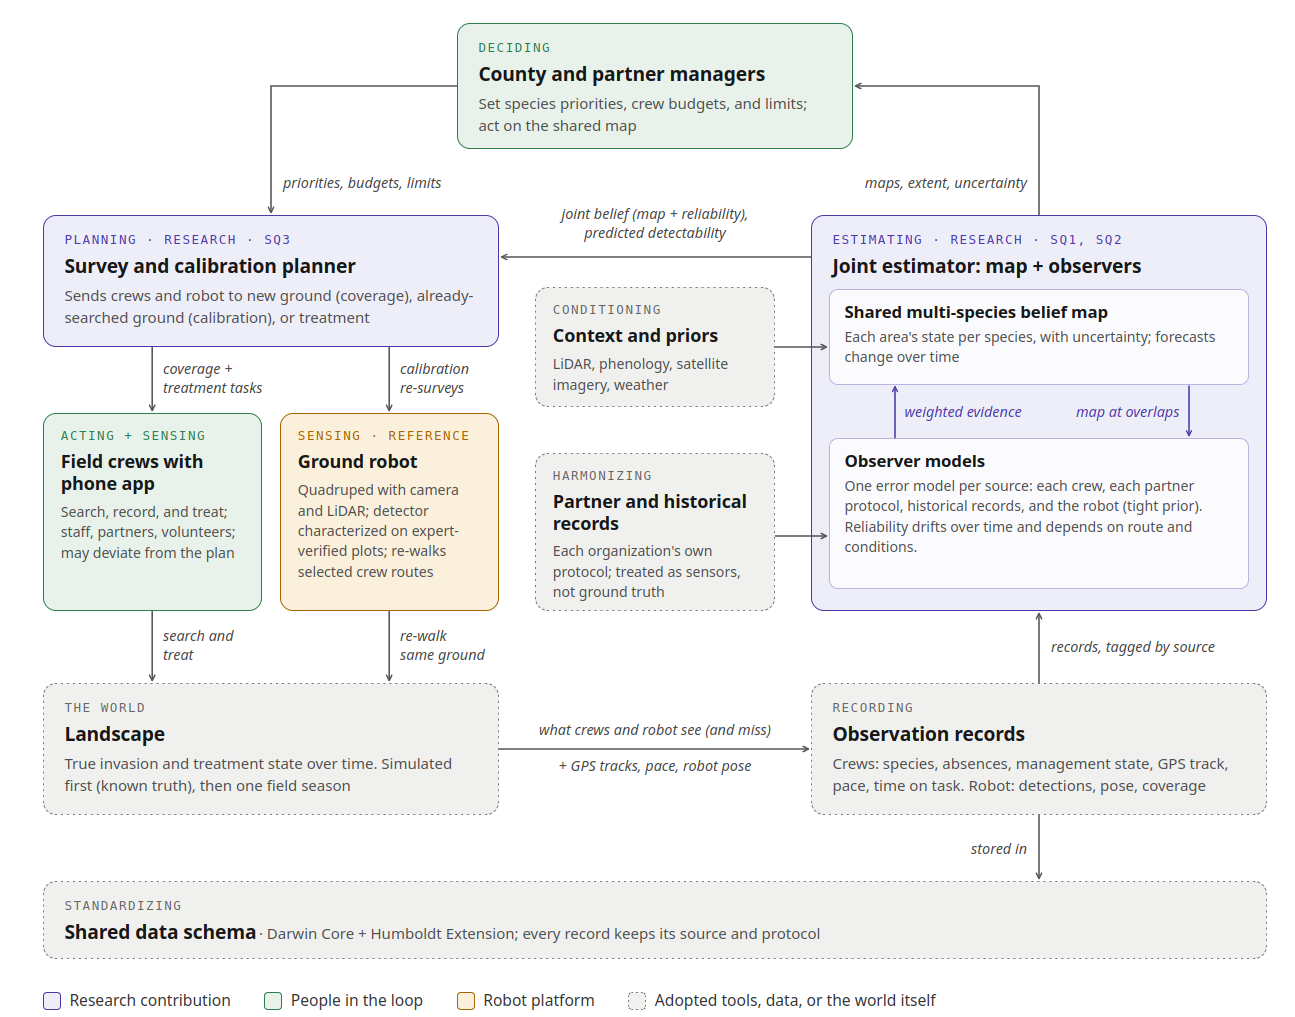
\includegraphics[width=\textwidth]{project-statement-diagram.png}
    \caption{High-level overview of the complete system including in-field data collection with both humans and a ground-based robot, probabilistic belief map generation, and county-wide decision making. The $SQ1$, $SQ2$, and $SQ3$ labels correspond to the respective sub-questions described above.}
    \label{fig:project-statement-diagram}
\end{figure*}

\clearpage

\bibliographystyle{IEEEtran}
\bibliography{references}

\end{document}
